\subsection{物理内存管理}
\subsubsection{Bitmap的实现}
物理内存需要通过一种数据结构来表示相应页是否已经分配,链表、数组等结构都可以胜任这个需求,但是还有一个更省空间的选择,那就是Bitmap. Bitmap表面上是一个字节指针,但是实际上一个页只对应着一位,即一个\texttt{char}型数据表示了三个页的分配情况.

本实验设计的Bitmap拥有数据开始地址和长度两个成员,而暴露出了三个接口分别用于获取位、置位以及完成一定长度内存页的申请(实际上是best-fit).代码实现如下:

\begin{figure}[H]
    \centering
    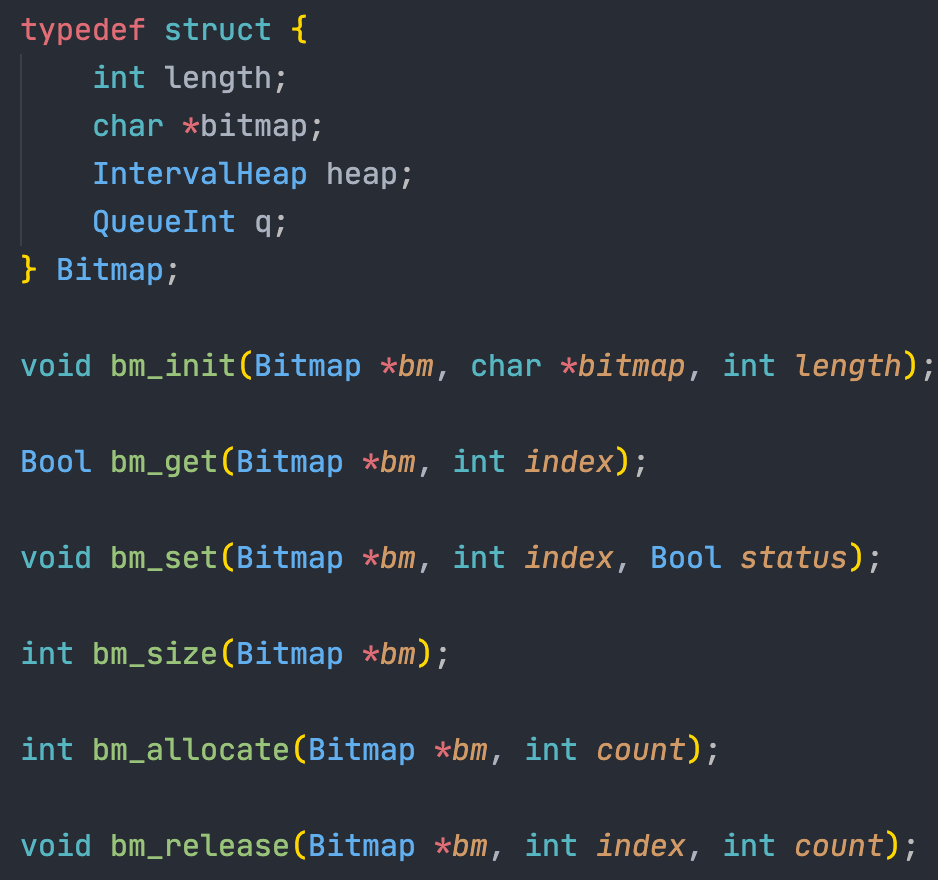
\includegraphics[width=\textwidth]{figures/bm0.png}
    \caption{Bitmap的数据结构}
    \label{fig:my_label}
\end{figure}

\begin{figure}[H]
    \centering
    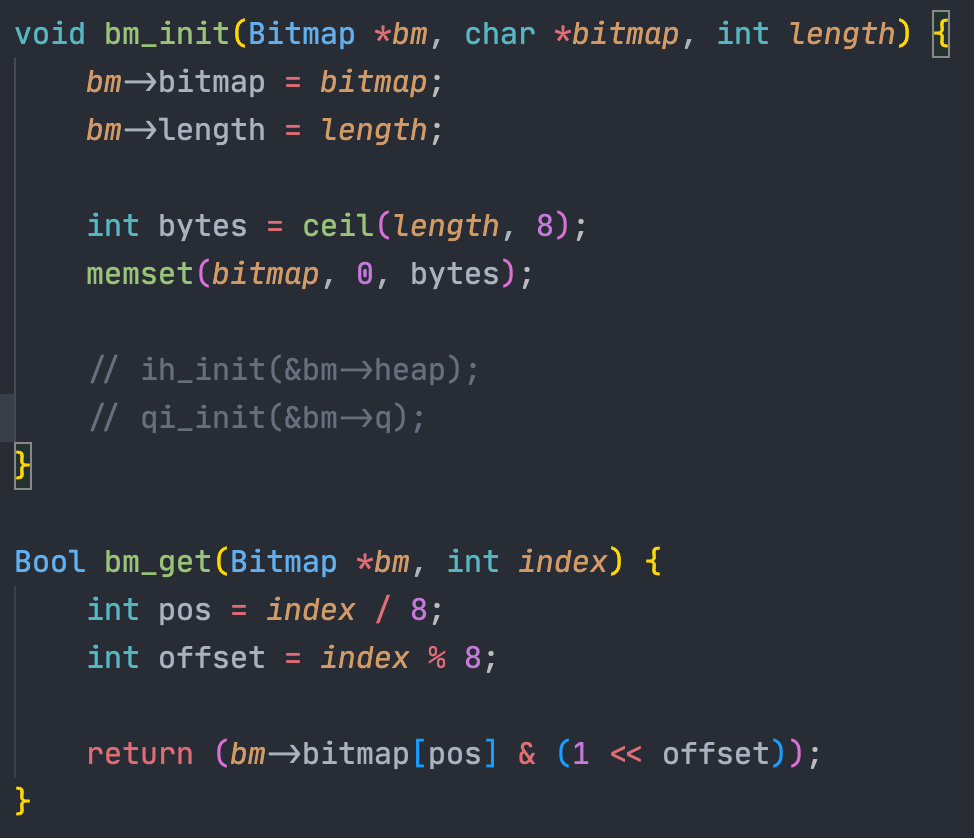
\includegraphics[width=0.8\textwidth]{figures/bm1.png}
    \caption{Bitmap初始化与get}
    \label{fig:my_label}
\end{figure}

\begin{figure}[H]
    \centering
    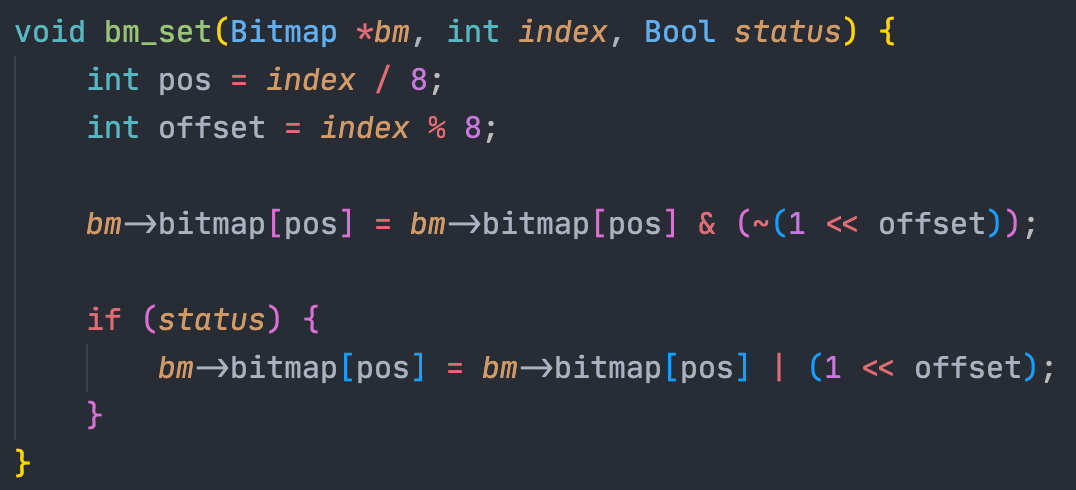
\includegraphics[width=\textwidth]{figures/bm2.png}
    \caption{set方法}
    \label{fig:my_label}
\end{figure}

\begin{figure}[H]
    \centering
    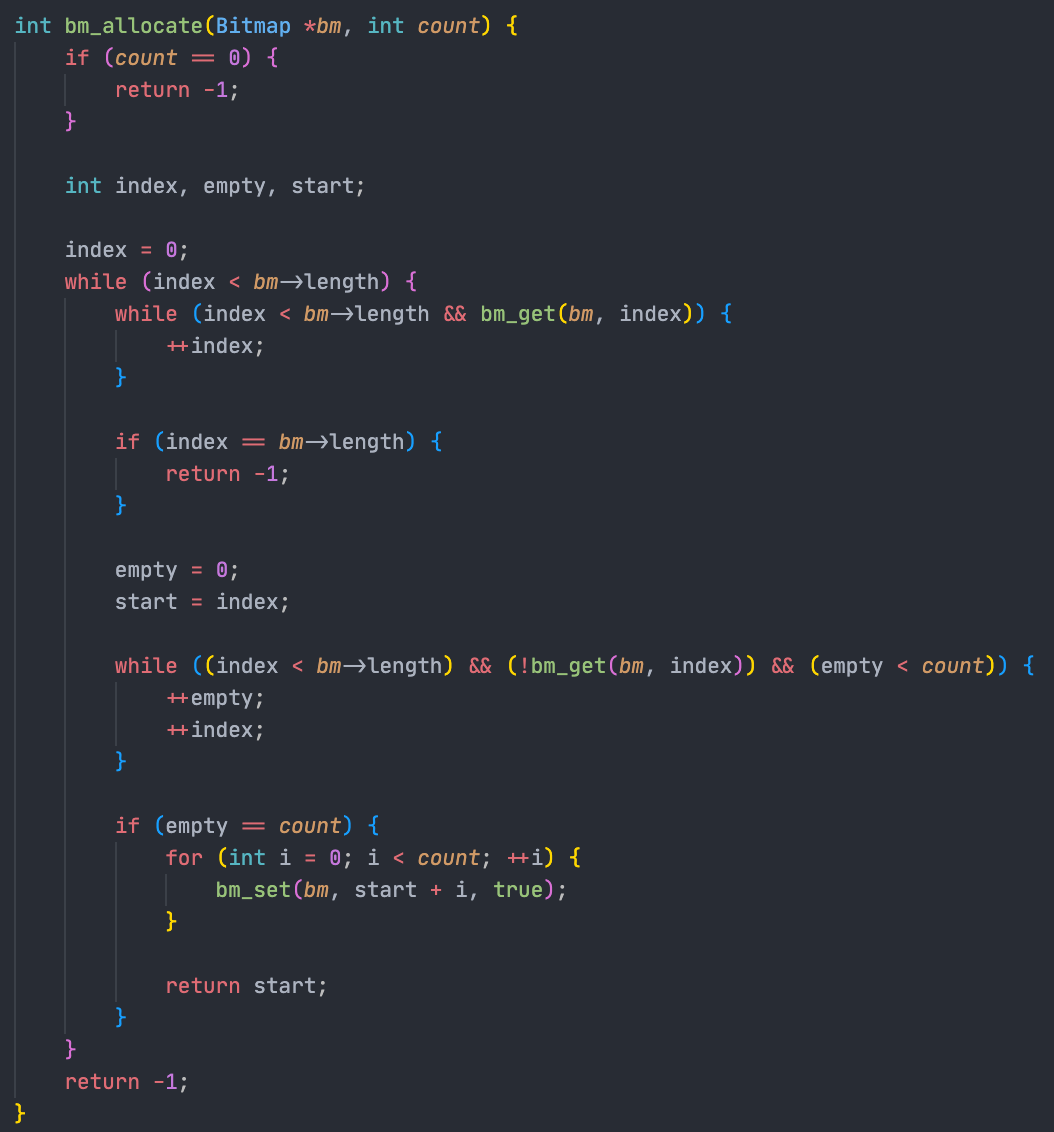
\includegraphics[width=\textwidth]{figures/bm3.png}
    \caption{分配与释放}
    \label{fig:my_label}
\end{figure}

\subsubsection{地址池的实现}
Bitmap之于内存就像PCB之于进程,只是方便理解与操作产生的产物,但这并不是真正的内存,所以我们需要将Bitmap中的位与实际中的内存地址进行对应,这就需要地址池了.

地址池具有基址和Bitmap两个成员,提供了申请若干页内存以及释放特定页内存两个接口.具体的功能就是将Bitmap中的索引乘上页长再加上基址得到实际分配内存页的起始地址.代码实现如下:

\begin{figure}[H]
    \centering
    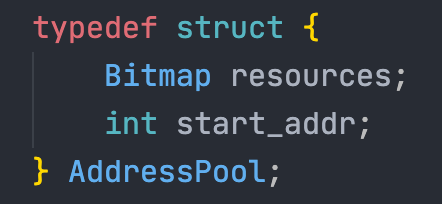
\includegraphics[width=0.4\textwidth]{figures/ap0.png}
    \caption{地址池数据结构}
    \label{fig:my_label}
\end{figure}

\begin{figure}[H]
    \centering
    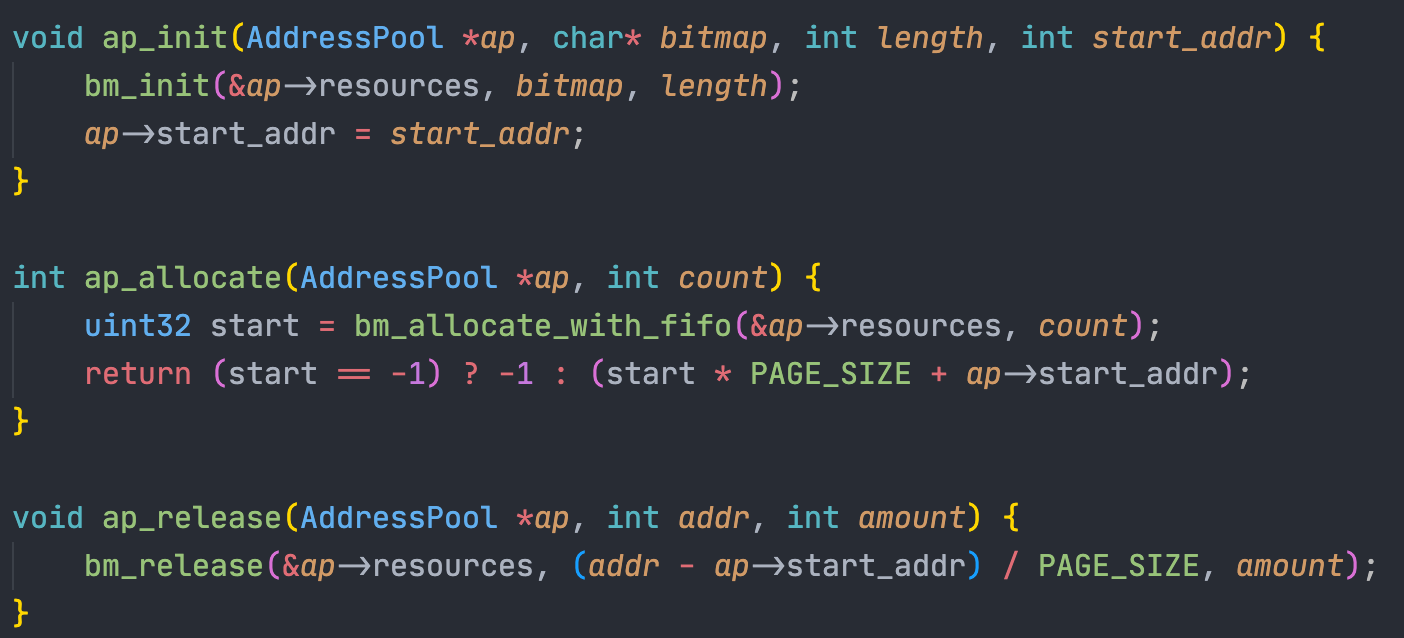
\includegraphics[width=\textwidth]{figures/ap1.png}
    \caption{地址池的方法}
    \label{fig:my_label}
\end{figure}

\subsubsection{内存管理器的实现}
现在我们获得了真正的地址,可以开始进行内存管理.

实际上地址空间分为内核地址和用户地址两种,所以在内存管理器中能够看到两种地址池.除此之外管理器进行的内存分配与释放操作也都是基于地址池完成的.值得注意的是,在内存管理器初始化的过程中,会利用通过mbr模式探查得到的总内存容量得到内存页数,其中一半分给内核地址(剩余一半分配给用户地址),并且将他们表示的连续空间基址安排在一个合适的地方.

\subsubsection{二级分页机制}
二级分页机制可以有效实现程序的动态重定位,避免了多个程序对相同的内存页的争夺.在x86的二级分页机制中,存在页表和页目录表二级分页,两种页均为4KiB大小. 32位地址被分为页目录项地址,页目录内页号和页内偏移量三个部分.

在具体实现上,二级分页机制的开启大概可以概括为以下几步:

\begin{enumerate}[itemindent=1em]
    \item 指定页目录表以及所有页表的地址,并进行初始化.
    \item 留出内存的前1MiB位置($\mathtt{0x00000000} \sim \mathtt{0x000fffff}$),这一段的虚拟地址就是真实地址,所以要在特定页表中给这一段内存留下``直通车''.
    \item 剩下的位置可以表示3GiB内存.其中第768个页表与第一个重复,页目录表最后一项指向本身,这是为了虚拟内存的实现.
    \item 最后要将页目录表地址置入\texttt{cr3}寄存器,且将\texttt{cr0}寄存器的PG位置\texttt{1},开启分页机制.
\end{enumerate}

代码实现如下:

\begin{figure}[H]
    \centering
    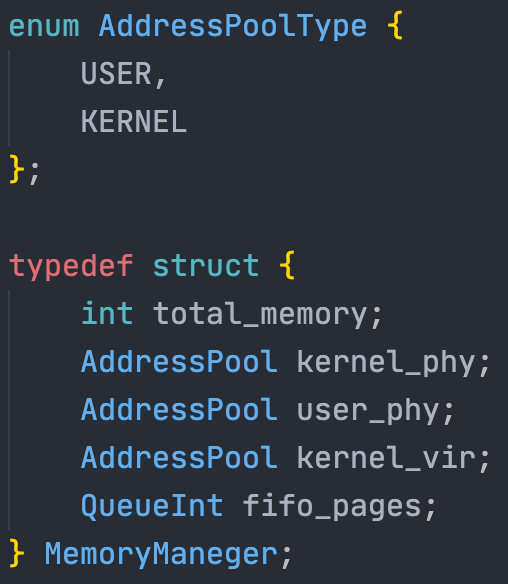
\includegraphics[width=0.4\textwidth]{figures/mm0.png}
    \caption{内存管理器的成员}
    \label{fig:my_label}
\end{figure}

\begin{figure}[H]
    \centering
    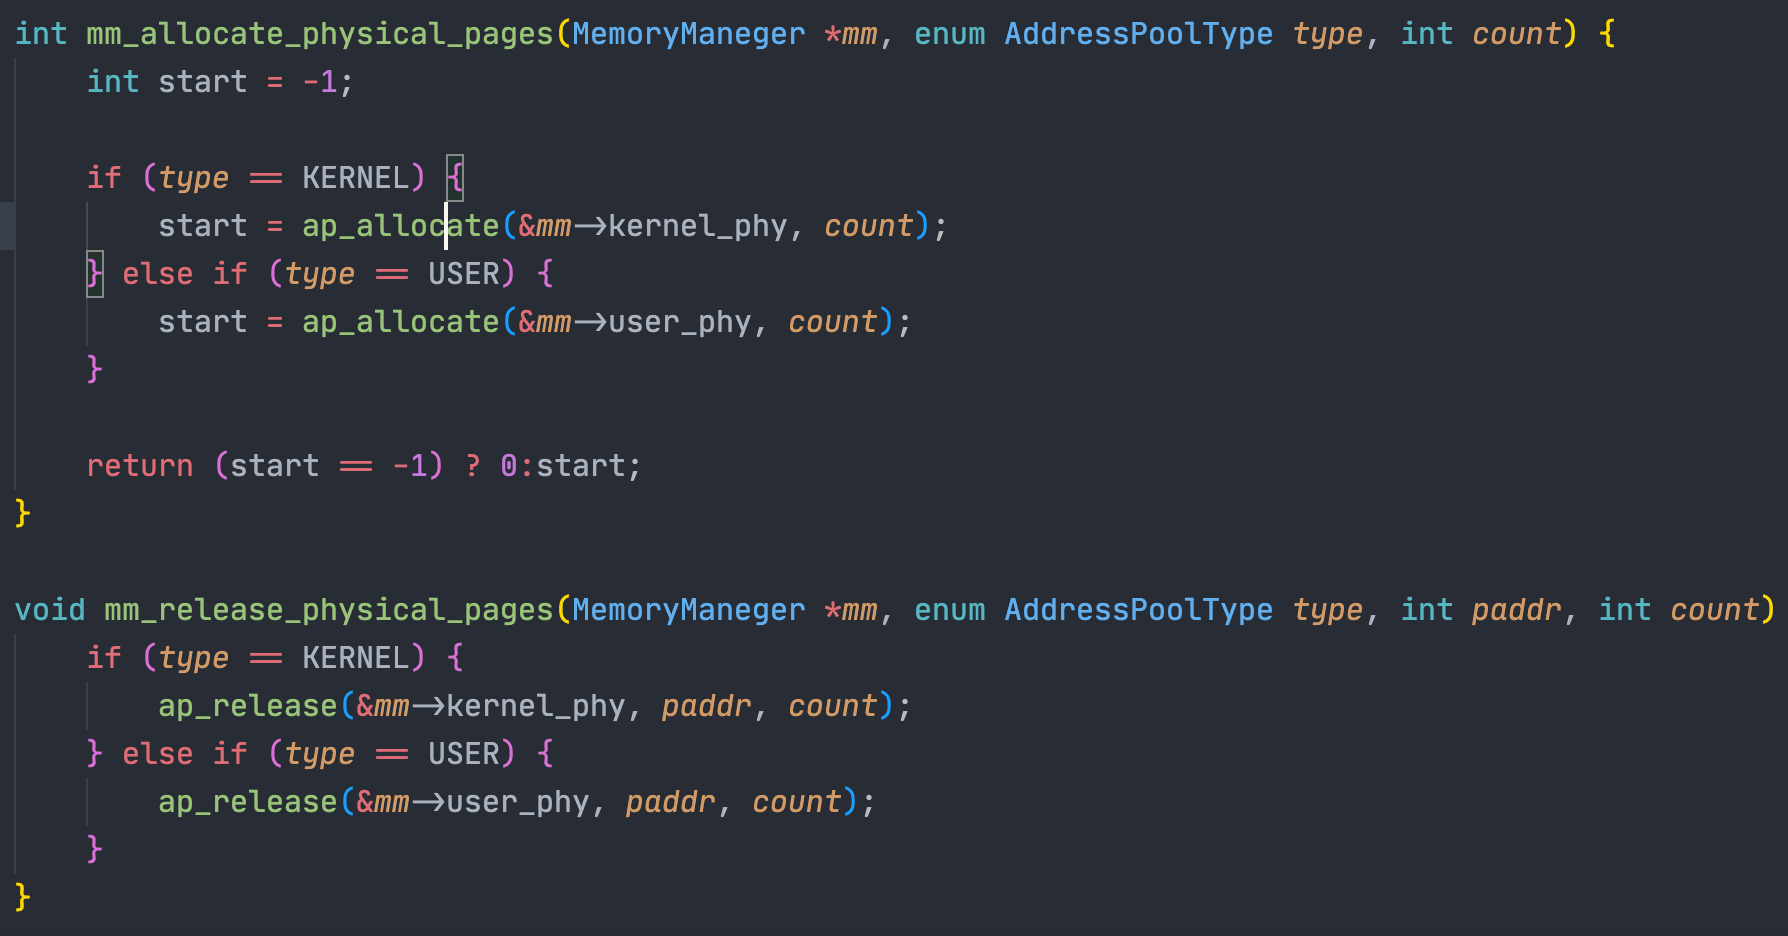
\includegraphics[width=\textwidth]{figures/mm1.png}
    \caption{内存管理器的分配与释放}
    \label{fig:my_label}
\end{figure}

\begin{figure}[H]
    \centering
    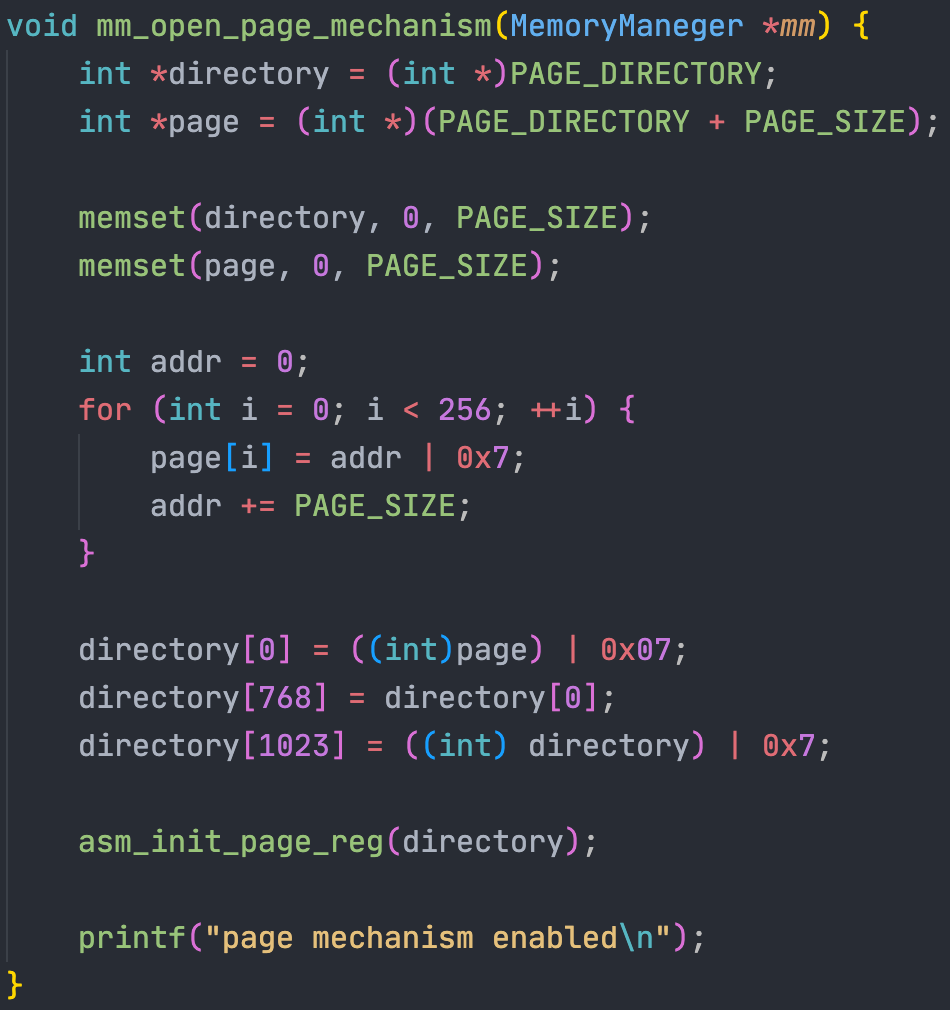
\includegraphics[width=0.8\textwidth]{figures/mm2.png}
    \caption{开启分页机制}
    \label{fig:my_label}
\end{figure}

综上,二级分页机制实现.

\subsection{动态内存分配}

本实验中选择实现worst-fit分配算法.

\subsubsection{算法原理}

worst-fit算法的原理非常简单,即选择内存中最大的一块空闲内存放置新分配的内存位置.这样可以有效降低外部碎片率,但是可能会导致大内存分配申请很难通过.使用这个算法需要时刻知道内存中最大的内存空隙是哪一个,因此需要维护一个极大堆优先队列.

\subsubsection{优先队列}

这里采用二叉堆来实现优先队列.这个数据结构已经在之前的课程中学习过,它能提供队列是否为空、压入成员以及弹出最大成员三个接口.代码实现如下:

\begin{figure}[H]
    \centering
    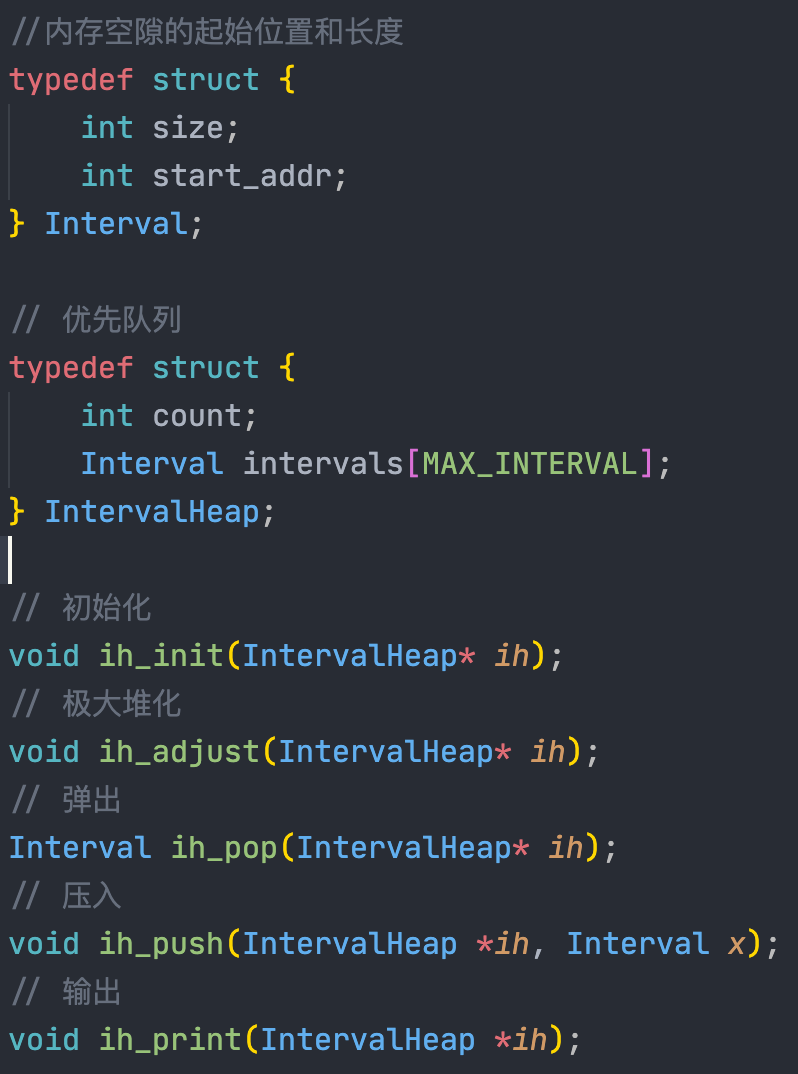
\includegraphics[width=0.8\textwidth]{figures/heap.png}
    \caption{优先队列成员以及方法(实现略)}
    \label{fig:my_label}
\end{figure}

\subsubsection{分配算法}

有了优先队列的辅助,分配算法就可以简单概括为:

\begin{enumerate}[itemindent=1em]
    \item 通过Bitmap获取各个空隙的长度和起始位置,一个个放进优先队列.
    \item 取出最大的空隙,返回其起始地址.
    \item 再次通过Bitmap获取空隙.
\end{enumerate}

代码实现如下:

\begin{figure}[H]
    \centering
    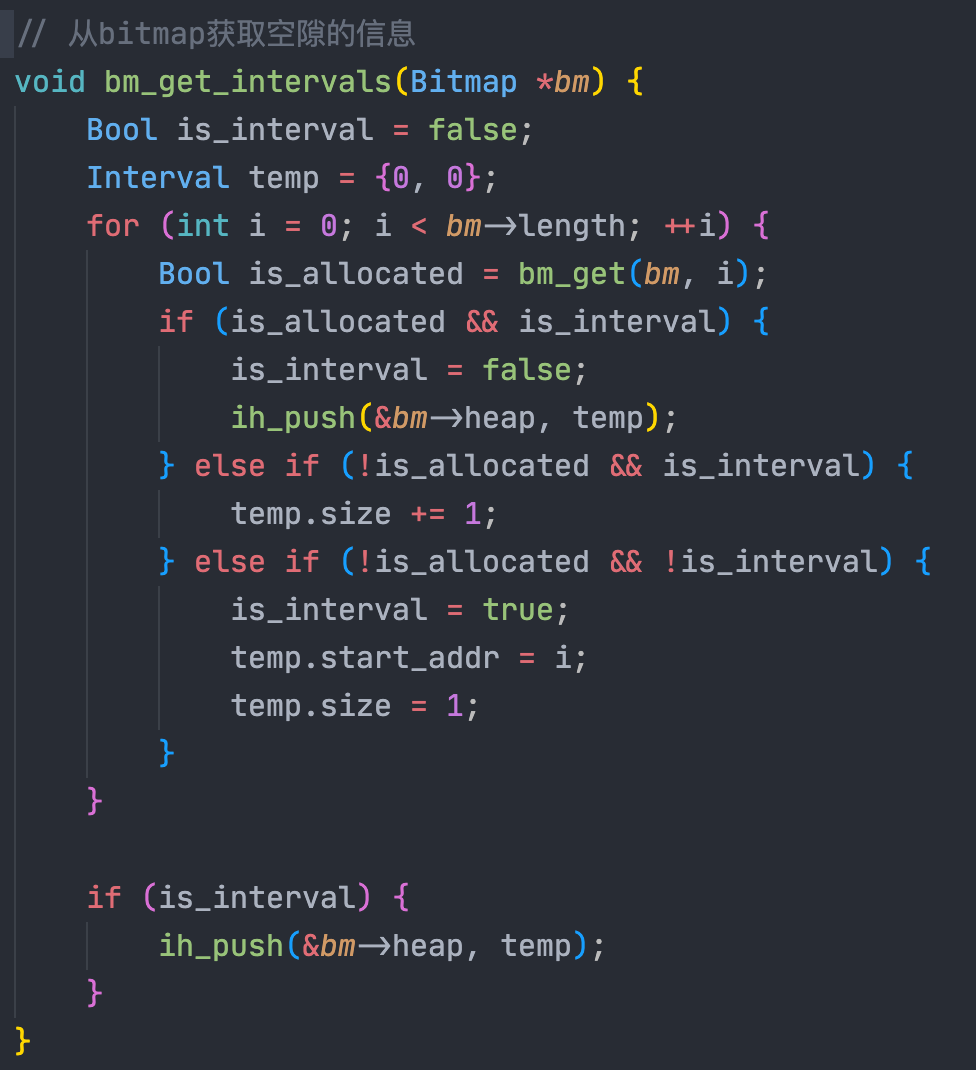
\includegraphics[width=0.8\textwidth]{figures/wf0.png}
    \caption{获取空隙信息}
    \label{fig:my_label}
\end{figure}

\begin{figure}[H]
    \centering
    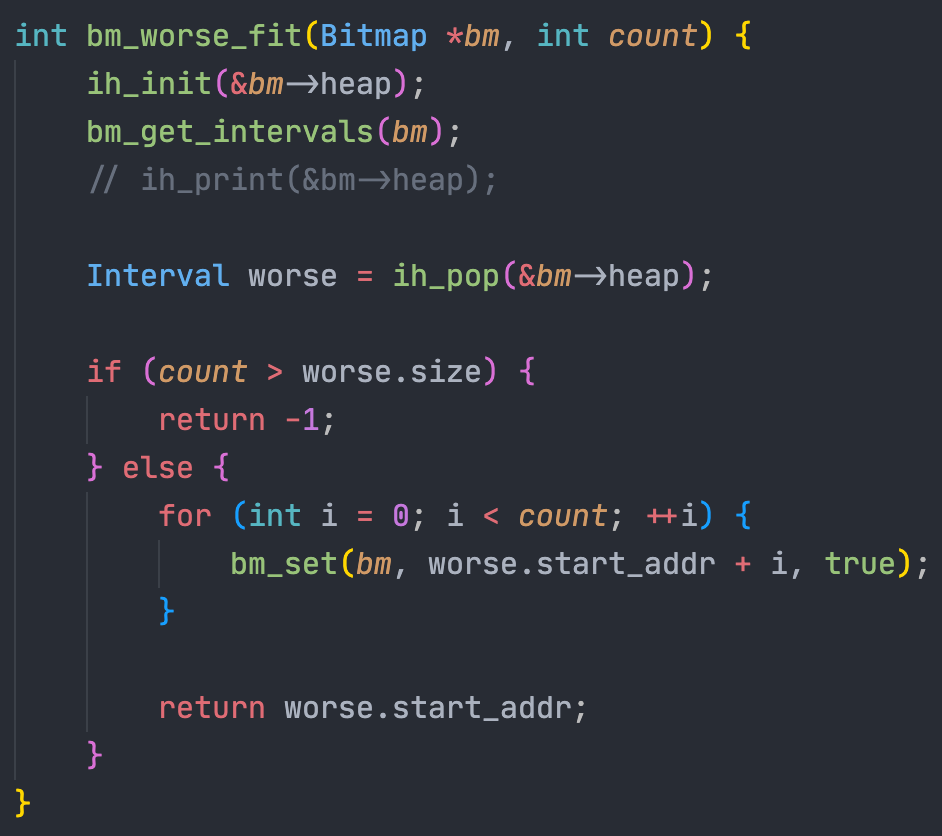
\includegraphics[width=0.8\textwidth]{figures/wf1.png}
    \caption{worst-fit主算法}
    \label{fig:my_label}
\end{figure}

从而, worst-fit的动态内存分配得到实现.

\subsection{页替换算法}

本实验采用较为简单的FIFO算法.即在页替换时首先弹出最先进入内存的页.算法需要一个队列维护.

\subsubsection{队列数据结构}

队列的实现不赘述,直接展示如何实现:

\begin{figure}[H]
    \centering
    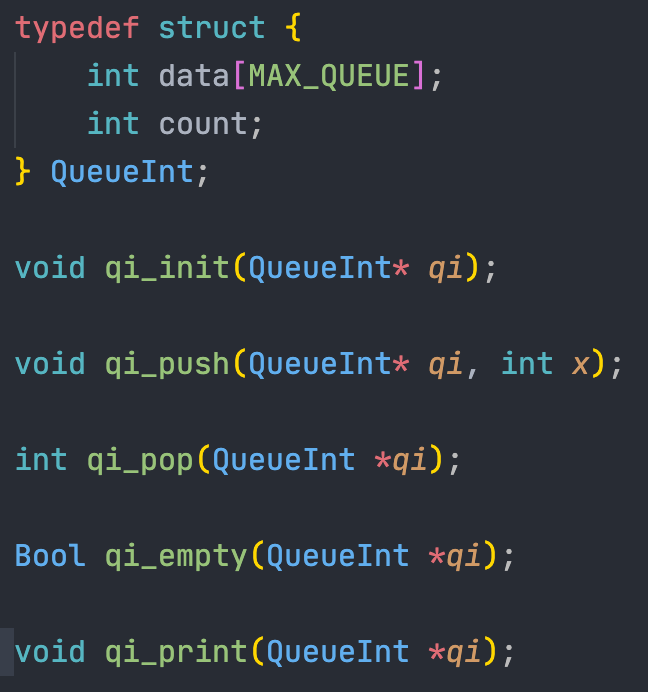
\includegraphics[width=0.4\textwidth]{figures/queue.png}
    \caption{队列数据结构与方法}
    \label{fig:my_label}
\end{figure}

\subsubsection{FIFO替换}

算法运行过程可以简要概括为:

\begin{enumerate}[itemindent=1em]
    \item 检测内存是否足够, 如果是直接分配内存,并将分配的内存页按页地址推入队列.
    \item 如果不够则一个个弹出并释放队首的页地址,直到空闲的内存能够满足此次分配申请.
\end{enumerate}

具体实现如下:

\begin{figure}[H]
    \centering
    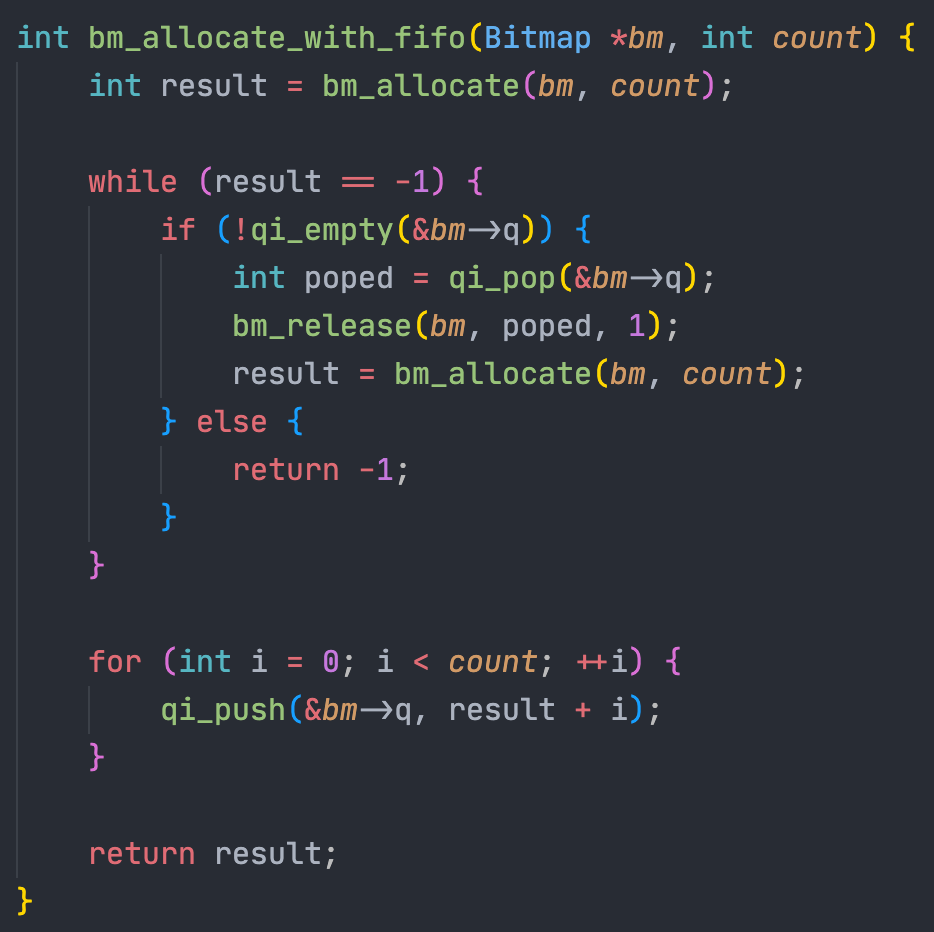
\includegraphics[width=0.8\textwidth]{figures/fifo.png}
    \caption{FIFO动态换页}
    \label{fig:my_label}
\end{figure}

\subsection{虚拟内存管理}

我们还可以采用虚拟内存的方式将增大我们所能管理的逻辑内存的空间.

\subsubsection{初始化}

虚拟内存自然需要一个地址池,这里添加一个新的内核虚拟地址池,内核虚拟空间起始地址是\texttt{0xc0100000}:

\subsubsection{分配}
过程如下:

\begin{enumerate}[itemindent=1em]
    \item 在虚拟地址池分配 $n$ 个连续的地址.
    \item 给这 $n$ 个虚拟地址各分配一个物理地址(不一定连续).
    \item 在页目录表和页表建立从虚拟地址到物理地址的一一对应.
\end{enumerate}

具体实现为:

\begin{figure}[H]
    \centering
    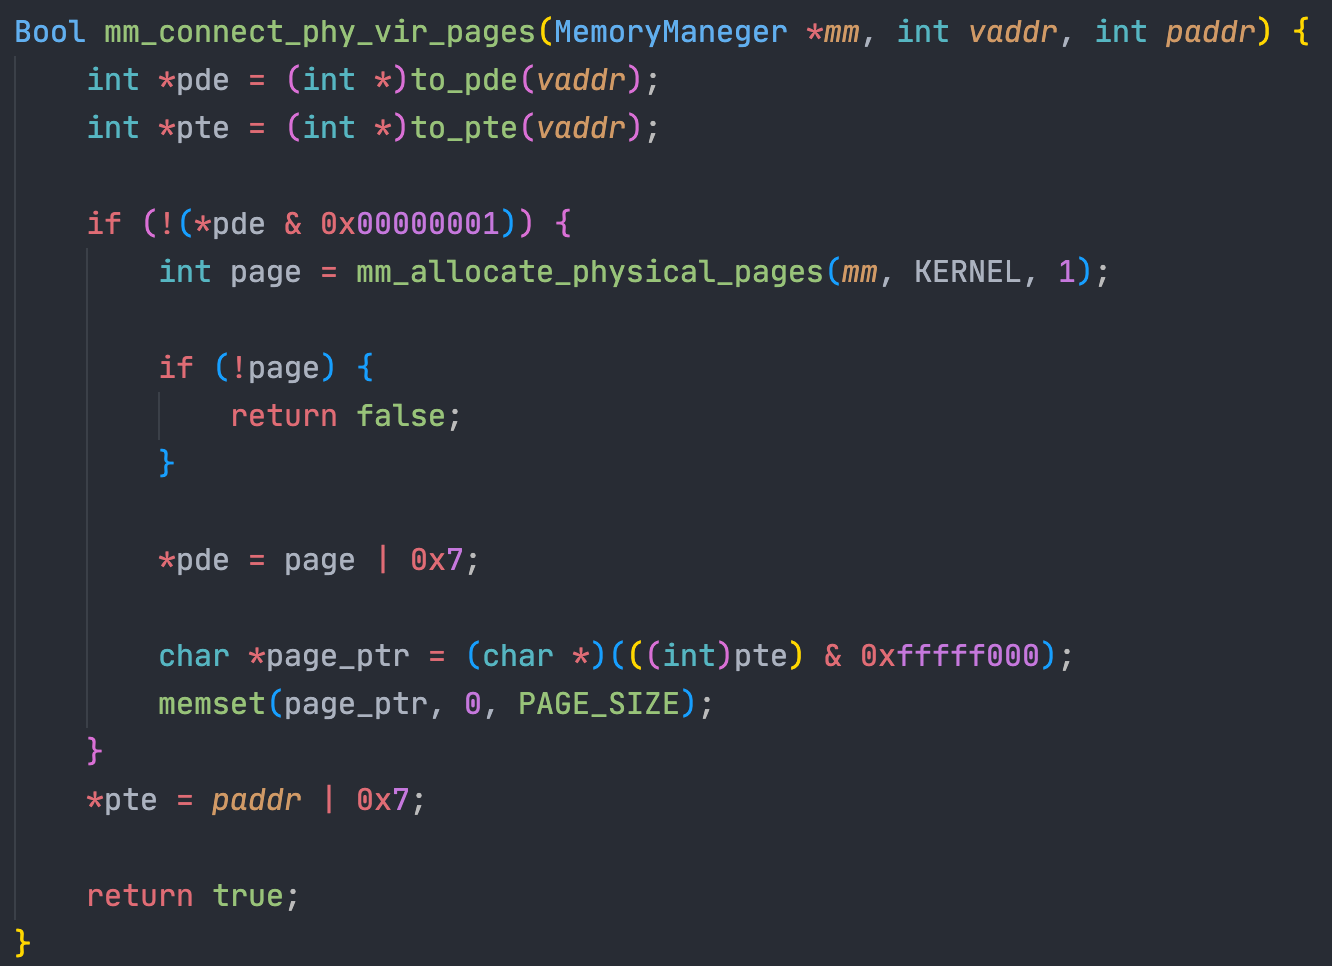
\includegraphics[width=\textwidth]{figures/va0.png}
    \caption{建立虚拟地址到物理地址的连接}
    \label{fig:my_label}
\end{figure}

\subsubsection{释放}
虚拟内存的释放流程如下:
\begin{enumerate}[itemindent=1em]
    \item 按照虚拟页号一个个释放对应的物理内存页.
    \item 释放虚拟页.
\end{enumerate}

\begin{figure}[H]
    \centering
    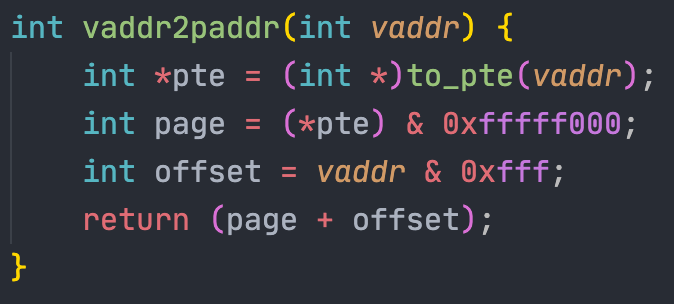
\includegraphics[width=0.6\textwidth]{figures/va1.png}
    \caption{地址转换}
    \label{fig:my_label}
\end{figure}

至此,虚拟内存管理机制已经完成.
